\documentclass[10pt,letterpaper]{article}
\usepackage[utf8]{inputenc}
\usepackage[T1]{fontenc}
\usepackage[provide=*,spanish]{babel}
\DeclareUnicodeCharacter{201C}{\textquotedblleft}
\DeclareUnicodeCharacter{201D}{\textquotedblright}
\usepackage[margin=2.2cm]{geometry}
\usepackage{amsmath,amssymb,booktabs,array,tabularx}
\usepackage{xcolor,tikz}
\usetikzlibrary{automata,positioning,arrows.meta}
\usepackage{hyperref}
\hypersetup{colorlinks=true,urlcolor=blue}
\usepackage{parskip}
\definecolor{navy}{RGB}{33,54,75}
\newcommand{\datos}[1]{\begin{center}{\Large\bfseries\color{navy}#1}\\[8pt]
Compiladores - Equipo 07\\Yañez Barajas Brandon - Model Designer\\2 de octubre de 2026\end{center}}
\newcommand{\tok}[1]{\texttt{#1}}
\begin{document}
\datos{Modelo AFND y AFD de tokens representativos}
\section*{1. Convenciones}
Modelé IDENTIFIER y CONSTANT a partir de las expresiones regulares de la especificación. La flecha de entrada indica el estado inicial y el doble círculo indica aceptación. Las transiciones omitidas en un AFND llegan al conjunto vacío. En las tablas de AFD, $M=\varnothing$ es el estado muerto y absorbe cualquier carácter.

\section*{2. Identificadores}
Patrón: \verb|[A-Za-z_][A-Za-z0-9_]*|. Defino $L$ como letra ASCII o guion bajo y $D$ como dígito. Un identificador requiere al menos un carácter de $L$.

\textbf{AFND.} $Q=\{q_0,q_1,q_2\}$, inicial $q_0$, finales $F=\{q_2\}$; alfabeto: caracteres de entrada, agrupados en $L$, $D$ y otros. Las transiciones no vacías son:
\[\delta(q_0,\varepsilon)=\{q_1\},\quad \delta(q_1,L)=\{q_2\},\quad
\delta(q_2,L)=\delta(q_2,D)=\{q_2\}.\]
\begin{center}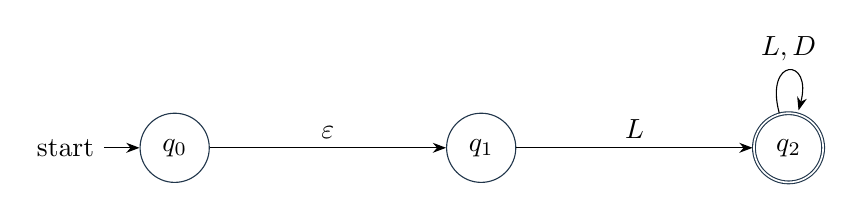
\begin{tikzpicture}[>=Stealth,node distance=3cm,every state/.style={draw=navy}]
\node[state,initial] (q0) {$q_0$}; \node[state,right=of q0] (q1) {$q_1$}; \node[state,accepting,right=of q1] (q2) {$q_2$};
\path[->] (q0) edge node[above] {$\varepsilon$} (q1) (q1) edge node[above] {$L$} (q2) (q2) edge[loop above] node {$L,D$} (q2);
\end{tikzpicture}\end{center}
\textbf{Clausuras.} $E(q_0)=\{q_0,q_1\}$, $E(q_1)=\{q_1\}$ y $E(q_2)=\{q_2\}$. La transición $\varepsilon$ no consume entrada.

\textbf{Subconjuntos.} El estado inicial del AFD es $A=E(\{q_0\})=\{q_0,q_1\}$. Al leer $L$, $E(\operatorname{mover}(A,L))=\{q_2\}=B$. Desde $B$, leer $L$ o $D$ conserva $B$. Un estado del AFD es final si contiene algún estado final del AFND; por eso $B$ es final.
\begin{center}\begin{tabular}{lccc}\toprule Estado & $L$ & $D$ & Otro\\\midrule
$\to A=\{q_0,q_1\}$ & $B$ & $M$ & $M$\\
$*B=\{q_2\}$ & $B$ & $B$ & $M$\\
$M=\varnothing$ & $M$ & $M$ & $M$\\\bottomrule\end{tabular}\end{center}
\begin{center}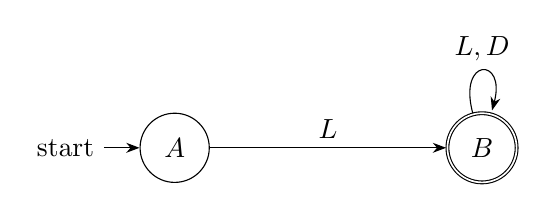
\begin{tikzpicture}[>=Stealth,node distance=3cm]
\node[state,initial] (a) {$A$}; \node[state,accepting,right=of a] (b) {$B$};
\path[->] (a) edge node[above] {$L$} (b) (b) edge[loop above] node {$L,D$} (b);
\end{tikzpicture}\end{center}
El diagrama muestra las transiciones principales; la tabla define también el estado muerto.
\textbf{Comprobación.} \tok{main}: $A\to B\to B\to B\to B$, aceptado. \tok{\_x} e \tok{if2} también se aceptan. \tok{2a}: $A\to M\to M$, rechazado; la cadena vacía queda en $A$, que no es final.

\newpage
\section*{3. Constantes numéricas}
Patrón: \verb|[0-9]+(\.[0-9]+)?|. Defino $d$ como dígito y el punto como carácter literal. Se aceptan enteros y decimales sin signo.

\textbf{AFND.} $Q=\{q_0,q_1,q_2,q_3,q_4,q_5\}$, inicial $q_0$, finales $F=\{q_2,q_5\}$. Las transiciones no vacías son:
\[\begin{aligned}
\delta(q_0,\varepsilon)&=\{q_1\}, & \delta(q_1,d)&=\{q_2\}, & \delta(q_2,d)&=\{q_2\},\\
\delta(q_2,\varepsilon)&=\{q_3\}, & \delta(q_3,\text{.})&=\{q_4\}, & \delta(q_4,d)&=\{q_5\},\\
\delta(q_5,d)&=\{q_5\}.&&&&
\end{aligned}\]
\begin{center}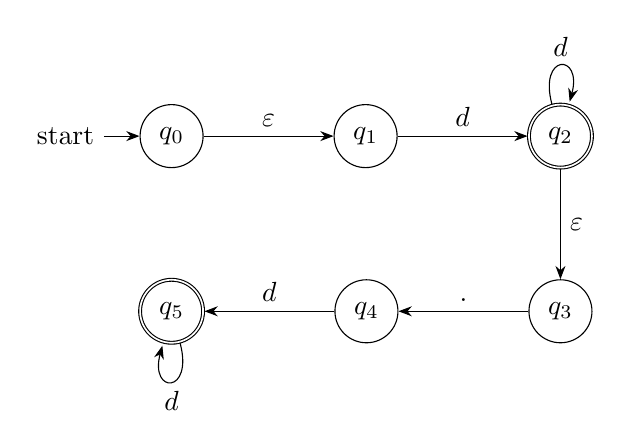
\begin{tikzpicture}[>=Stealth,node distance=1.65cm,every state/.style={minimum size=8mm,inner sep=1pt}]
\node[state,initial] (q0) {$q_0$}; \node[state,right=of q0] (q1) {$q_1$}; \node[state,accepting,right=of q1] (q2) {$q_2$};
\node[state,below=1.4cm of q2] (q3) {$q_3$}; \node[state,left=of q3] (q4) {$q_4$}; \node[state,accepting,left=of q4] (q5) {$q_5$};
\path[->] (q0) edge node[above] {$\varepsilon$} (q1) (q1) edge node[above] {$d$} (q2) (q2) edge[loop above] node {$d$} (q2)
(q2) edge node[right] {$\varepsilon$} (q3) (q3) edge node[above] {.} (q4) (q4) edge node[above] {$d$} (q5) (q5) edge[loop below] node {$d$} (q5);
\end{tikzpicture}\end{center}
\textbf{Clausuras.} $E(q_0)=\{q_0,q_1\}$, $E(q_2)=\{q_2,q_3\}$. Para $q_1,q_3,q_4,q_5$, la clausura contiene únicamente el propio estado.

\textbf{Subconjuntos.} $S=\{q_0,q_1\}$ es inicial. $E(\operatorname{mover}(S,d))=\{q_2,q_3\}=N$. Desde $N$, un dígito conserva $N$ y un punto llega a $P=\{q_4\}$. Desde $P$, un dígito llega a $F_d=\{q_5\}$; los dígitos posteriores conservan $F_d$. $N$ y $F_d$ son finales porque contienen $q_2$ y $q_5$, respectivamente.
\begin{center}\begin{tabular}{lccc}\toprule Estado & $d$ & Punto & Otro\\\midrule
$\to S=\{q_0,q_1\}$ & $N$ & $M$ & $M$\\
$*N=\{q_2,q_3\}$ & $N$ & $P$ & $M$\\
$P=\{q_4\}$ & $F_d$ & $M$ & $M$\\
$*F_d=\{q_5\}$ & $F_d$ & $M$ & $M$\\
$M=\varnothing$ & $M$ & $M$ & $M$\\\bottomrule\end{tabular}\end{center}
\begin{center}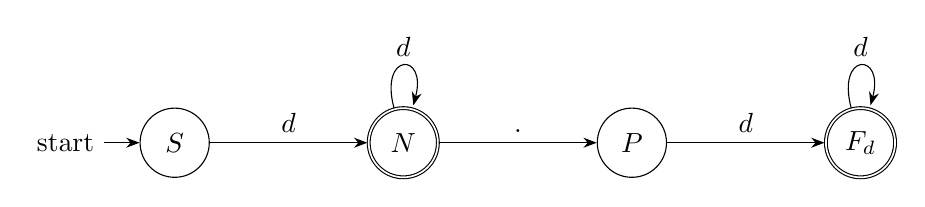
\begin{tikzpicture}[>=Stealth,node distance=2cm]
\node[state,initial] (s) {$S$}; \node[state,accepting,right=of s] (n) {$N$}; \node[state,right=of n] (p) {$P$}; \node[state,accepting,right=of p] (f) {$F_d$};
\path[->] (s) edge node[above] {$d$} (n) (n) edge[loop above] node {$d$} (n) (n) edge node[above] {.} (p) (p) edge node[above] {$d$} (f) (f) edge[loop above] node {$d$} (f);
\end{tikzpicture}\end{center}
\textbf{Comprobación.} \tok{10}: $S\to N\to N$, aceptado. \tok{3.14}: $S\to N\to P\to F_d\to F_d$, aceptado. \tok{3.} termina en $P$, no final; \tok{123abc} y \tok{1.2.3} llegan a $M$ y se rechazan como constantes completas.

\section*{4. Relación con el lexer}
Los autómatas describen los mismos lenguajes regulares que los patrones del programa. Aunque la implementación use regex, este modelo conserva la conversión por clausuras y subconjuntos vista en clase. La aceptación aquí evalúa un candidato completo; el lexer además identifica sus límites, aplica la coincidencia más larga y reporta errores. Un identificador reservado se reclasifica como KEYWORD; \tok{-10} se separa en operador y constante.

\end{document}
